\chapter*{ประวัติผู้เขียน}
\addcontentsline{toc}{chapter}{ประวัติผู้เขียน}
\label{chap:biography}

\vspace{0.2cm}

\noindent
\begin{minipage}[c]{0.26\textwidth}
    \centering
    \begin{tikzpicture}
        \fill[black!15] (0.04,-0.04) circle (1.25cm);
        \node[circle, draw=quantumGold, line width=2pt, inner sep=0pt] at (0,0) {
            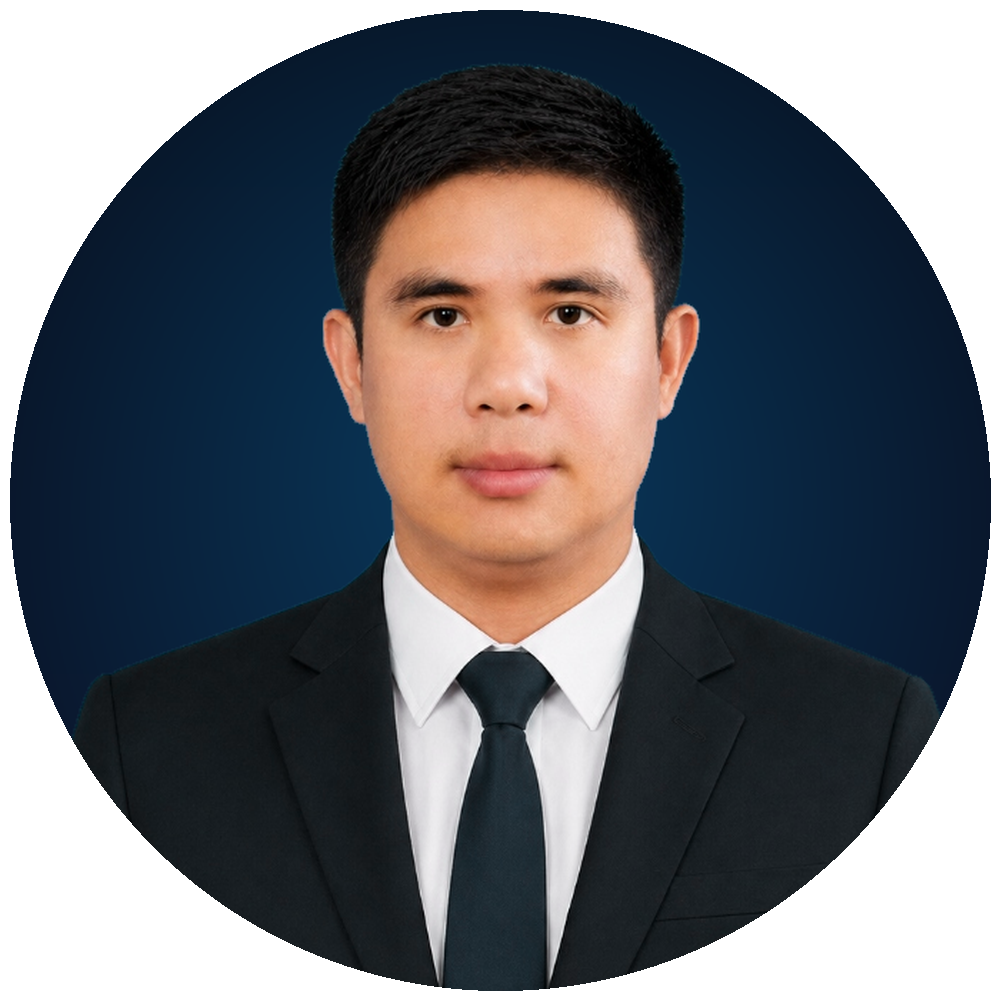
\includegraphics[width=2.4cm,height=2.4cm,keepaspectratio]{images/author_chewa_circle_final.png}
        };
    \end{tikzpicture}
\end{minipage}\hfill
\begin{minipage}[c]{0.71\textwidth}
    {\fontsize{16}{20}\selectfont\bfseries\color{darkNavy} ผู้ช่วยศาสตราจารย์ ดร.ชีวะ ทัศนา}\\[0.15cm]
    {\fontsize{11}{15}\selectfont
    สาขาวิชาฟิสิกส์ คณะวิทยาศาสตร์และเทคโนโลยี\\
    มหาวิทยาลัยราชภัฏรำไพพรรณี\\[0.05cm]
    \textbf{อีเมล}\ \texttt{chewa.t@rbru.ac.th}\\
    \textbf{เว็บไซต์วิชาการ}\ \url{https://science.rbru.ac.th}}
\end{minipage}

\vspace{0.15cm}
{\color{cyberBlue!30}\hrule height 0.8pt}
\vspace{0.15cm}

\noindent
\begin{minipage}[t]{0.48\textwidth}
    {\fontsize{12}{15}\selectfont\bfseries\color{cyberBlue} ประวัติการศึกษา}\par\vspace{2pt}
    \begin{itemize}\setlength{\itemsep}{1pt}\setlength{\parsep}{0pt}\setlength{\topsep}{1pt}\setlength{\partopsep}{0pt}\setlength{\leftmargin}{12pt}
        \item \textbf{ปร.ด. (ฟิสิกส์ประยุกต์)}\\Ph.D. in Applied Physics
        \item \textbf{วท.ม. (ฟิสิกส์ประยุกต์)}\\M.Sc. in Applied Physics
        \item \textbf{วท.บ. (ฟิสิกส์ คอมพิวเตอร์และอิเล็กทรอนิกส์)}\\B.Sc. in Physics, Computer and Electronics
    \end{itemize}

    \vspace{0.2cm}
    {\fontsize{12}{15}\selectfont\bfseries\color{cyberBlue} ภาระงานสอนประจำ}\par\vspace{2pt}
    \begin{itemize}\setlength{\itemsep}{1pt}\setlength{\parsep}{0pt}\setlength{\topsep}{1pt}\setlength{\partopsep}{0pt}\setlength{\leftmargin}{12pt}
        \item ฟิสิกส์แผนใหม่ (Modern Physics)
        \item คณิตศาสตร์สำหรับฟิสิกส์ (Mathematics for Physics)
        \item ฟิสิกส์เชิงคำนวณและการจำลองด้วยคอมพิวเตอร์ (Computational Physics)
        \item ปฏิบัติการฟิสิกส์ขั้นสูง (Advanced Physics Laboratory)
    \end{itemize}
\end{minipage}\hfill
\begin{minipage}[t]{0.49\textwidth}
    {\fontsize{12}{15}\selectfont\bfseries\color{neonPurple} ความเชี่ยวชาญและงานวิจัยที่สนใจ}\par\vspace{2pt}
    \begin{itemize}\setlength{\itemsep}{2pt}\setlength{\parsep}{0pt}\setlength{\topsep}{1pt}\setlength{\partopsep}{0pt}\setlength{\leftmargin}{12pt}
        \item การจำลองปรากฏการณ์ฟิสิกส์เสมือนจริงด้วย WebXR, AR และ Spatial Computing
        \item ระเบียบวิธีเชิงตัวเลขและวิทยาการคอมพิวเตอร์ควอนตัม (Quantum Computing \& Simulation)
        \item การพัฒนาระบบ Active Learning และสื่อจำลองเชิงโต้ตอบ 60 FPS บนเว็บและคลาวด์
        \item การประยุกต์ปัญญาประดิษฐ์ (AI) ในการวิเคราะห์ข้อมูลฟิสิกส์และการสร้างสื่อการเรียนรู้ขั้นสูง
    \end{itemize}
\end{minipage}

